\documentclass[conference]{IEEEtran}
\IEEEoverridecommandlockouts

\usepackage{cite}
\usepackage{amsmath,amssymb,amsfonts}
\usepackage{algorithmic}
\usepackage{graphicx}
\usepackage{textcomp}
\usepackage{xcolor}
\usepackage{booktabs}
\usepackage{url}

\def\BibTeX{{\rm B\kern-.05em{\sc i\kern-.025em b}\kern-.08em
    T\kern-.1667em\lower.7ex\hbox{E}\kern-.125emX}}

\begin{document}

\title{Drift-Aware Behavioral Anomaly Detection: Mitigating Poisoning Attacks in Adaptive Insider Threat Detection\\
{\footnotesize \textsuperscript{*}Department of Computer Science and Engineering, Final Year Major Project}
}

\author{\IEEEauthorblockN{Mahisha V}
\IEEEauthorblockA{\textit{Department of Computer Science and Engineering} \\
\textit{Your College / University Name}\\
City, State, India \\
mahisha.v@example.edu}
\and
\IEEEauthorblockN{Project Guide / Faculty Advisor}
\IEEEauthorblockA{\textit{Department of Computer Science and Engineering} \\
\textit{Your College / University Name}\\
City, State, India \\
guide.email@example.edu}
}

\maketitle

\begin{abstract}
Insider threats represent one of the most critical challenges in modern enterprise cybersecurity, as malicious insiders already possess legitimate credentials and authorized access to organizational assets. While User and Entity Behavior Analytics (UEBA) systems leverage unsupervised anomaly detection techniques such as Isolation Forests, they confront a fundamental dilemma in dynamic operational environments. Static detection models fail to accommodate benign operational evolution, causing excessive false positive rates. Conversely, naive adaptive models employing exponential moving average (EMA) updates are vulnerable to adversarial concept drift—a gradual poisoning strategy where adversaries incrementally escalate anomalous activities to blend into the shifting baseline. In this paper, we propose a Drift-Aware Behavioral Anomaly Detection framework equipped with an automated Z-score sum persistence lock mechanism. Our architecture ingests continuous multi-vector endpoint telemetry—including process execution, network volume deltas, session durations, and physical USB peripheral interactions verified at the operating system kernel level. When cumulative feature deviation exceeds an empirical statistical threshold ($\sum |Z| \ge 4.5$), the system locks baseline adaptation, preventing adversary-induced model poisoning while preserving legitimate drift adaptation. We conduct a rigorous 30-trial empirical evaluation across four distinct drift stress levels. The proposed Drift-Aware model sustains an F1-score of $0.968 \pm 0.023$ under severe adversarial drift, compared to $0.503$ achieved by the naive adaptive baseline ($p = 0.0001$), confirming statistically significant resilience against behavioral poisoning attacks.
\end{abstract}

\begin{IEEEkeywords}
Insider Threat Detection, User and Entity Behavior Analytics (UEBA), Concept Drift, Isolation Forest, Adversarial Poisoning, Endpoint Telemetry.
\end{IEEEkeywords}

\section{Introduction}
Modern enterprise cybersecurity perimeters are increasingly vulnerable to malicious insider actions. According to recent threat intelligence reports, insider-driven incidents have surged by over 44\% in frequency, with the average incident remediation cost exceeding \$15 million \cite{b1}. Unlike external attackers attempting unauthorized network penetration, malicious insiders (including disaffected employees, compromised privileged accounts, and industrial espionage agents) operate with valid authentication credentials and routine data access privileges. Consequently, perimeter-based defenses—such as firewalls, intrusion prevention systems (IPS), and signature-driven antivirus solutions—frequently fail to identify authorized users conducting unauthorized data exfiltration or privilege escalation \cite{b2}.

To counteract this vulnerability, User and Entity Behavior Analytics (UEBA) architectures utilize unsupervised machine learning algorithms to establish normative behavioral baselines for each employee or entity \cite{b3}. Algorithms such as Isolation Forests \cite{b4} isolate anomalous feature instances without requiring exhaustively labeled attack datasets, which are notoriously scarce in insider threat domains.

However, existing UEBA systems suffer from a critical operational challenge: \textit{the adaptation-poisoning dilemma} \cite{b5}. Real-world employee behaviors naturally evolve over time due to seasonal project demands, organizational restructuring, and shifting working hours. If an anomaly detection model remains \textit{static}, it cannot accommodate benign behavioral evolution, resulting in an unsustainable rate of false alarms that overwhelms security operations center (SOC) analysts. 

Conversely, if the detection engine adopts a \textit{naive adaptive} approach—incrementally updating its behavioral baseline using Exponential Moving Averages (EMA) or sliding windows—it introduces an attack vector known as \textit{adversarial concept drift} or \textit{boiling frog attacks} \cite{b6}. A sophisticated insider can gradually escalate unauthorized data copying and off-hours activity over weeks or months. Under naive adaptation, the model incorporates these subtle malicious increments into its normative baseline, effectively learning to recognize malicious exfiltration as standard operational behavior.

To resolve this dilemma, this paper presents a novel \textbf{Drift-Aware Behavioral Anomaly Detection Framework} featuring:
\begin{enumerate}
    \item \textbf{Kernel-Verified Endpoint Sensor:} A real-time hardware telemetry agent that captures authentic process executions, network deltas, and physical USB flash storage drive attachments verified via Windows Kernel system calls (\texttt{GetDriveTypeW}).
    \item \textbf{Statistical Persistence Lock Mechanism:} A drift detector tracking cumulative Z-score deviations across an orthogonal 6-dimensional behavioral vector. When multi-feature drift crosses a statistical significance threshold ($\sum |Z| \ge 4.5$), baseline parameter updates are locked, stopping adversarial poisoning.
    \item \textbf{Empirical 30-Trial Comparative Validation:} A statistical evaluation assessing Static, Naive Adaptive, and Drift-Aware models across four drift stress levels with paired $t$-tests ($p < 0.05$).
\end{enumerate}

\section{Related Work}
\subsection{Insider Threat Detection and UEBA}
Insider threat detection frameworks historically relied on rule-based policy engines and audit log parsing \cite{b2}. Modern methodologies transition toward data-driven UEBA architectures utilizing unsupervised clustering, autoencoders, and tree-based isolation ensembles \cite{b3}, \cite{b7}. Liu et al. demonstrated that Isolation Forests outperform traditional distance-based methods like Local Outlier Factor (LOF) and One-Class SVMs in high-dimensional telemetry environments due to their linear time complexity and minimal memory footprint \cite{b4}.

\subsection{Concept Drift and Adversarial Poisoning}
Concept drift denotes statistical shifts in data distributions over time ($P_t(X, y) \neq P_{t+1}(X, y)$) \cite{b5}. In security-sensitive anomaly detection, concept drift bifurcates into benign drift (legitimate operational shifts) and adversarial drift (adversaries deliberately polluting training baselines) \cite{b6}. Kloft and Laskov analyzed online learning vulnerabilities under poisoning attacks, demonstrating that unconstrained online updates guarantee bounded evasion success for persistent adversaries \cite{b8}. Existing mitigation techniques commonly deploy decay windows or dual-memory ensembles; however, these approaches lack explicit statistical locking mechanisms triggered by cumulative multi-vector behavioral anomalies.

\section{System Architecture and Methodology}
The implemented architecture follows a distributed microservices paradigm consisting of an endpoint telemetry sensor, an inference microservice, an enterprise API gateway, and a visualization console (Fig.~\ref{fig:arch}).

\begin{figure}[htbp]
\centerline{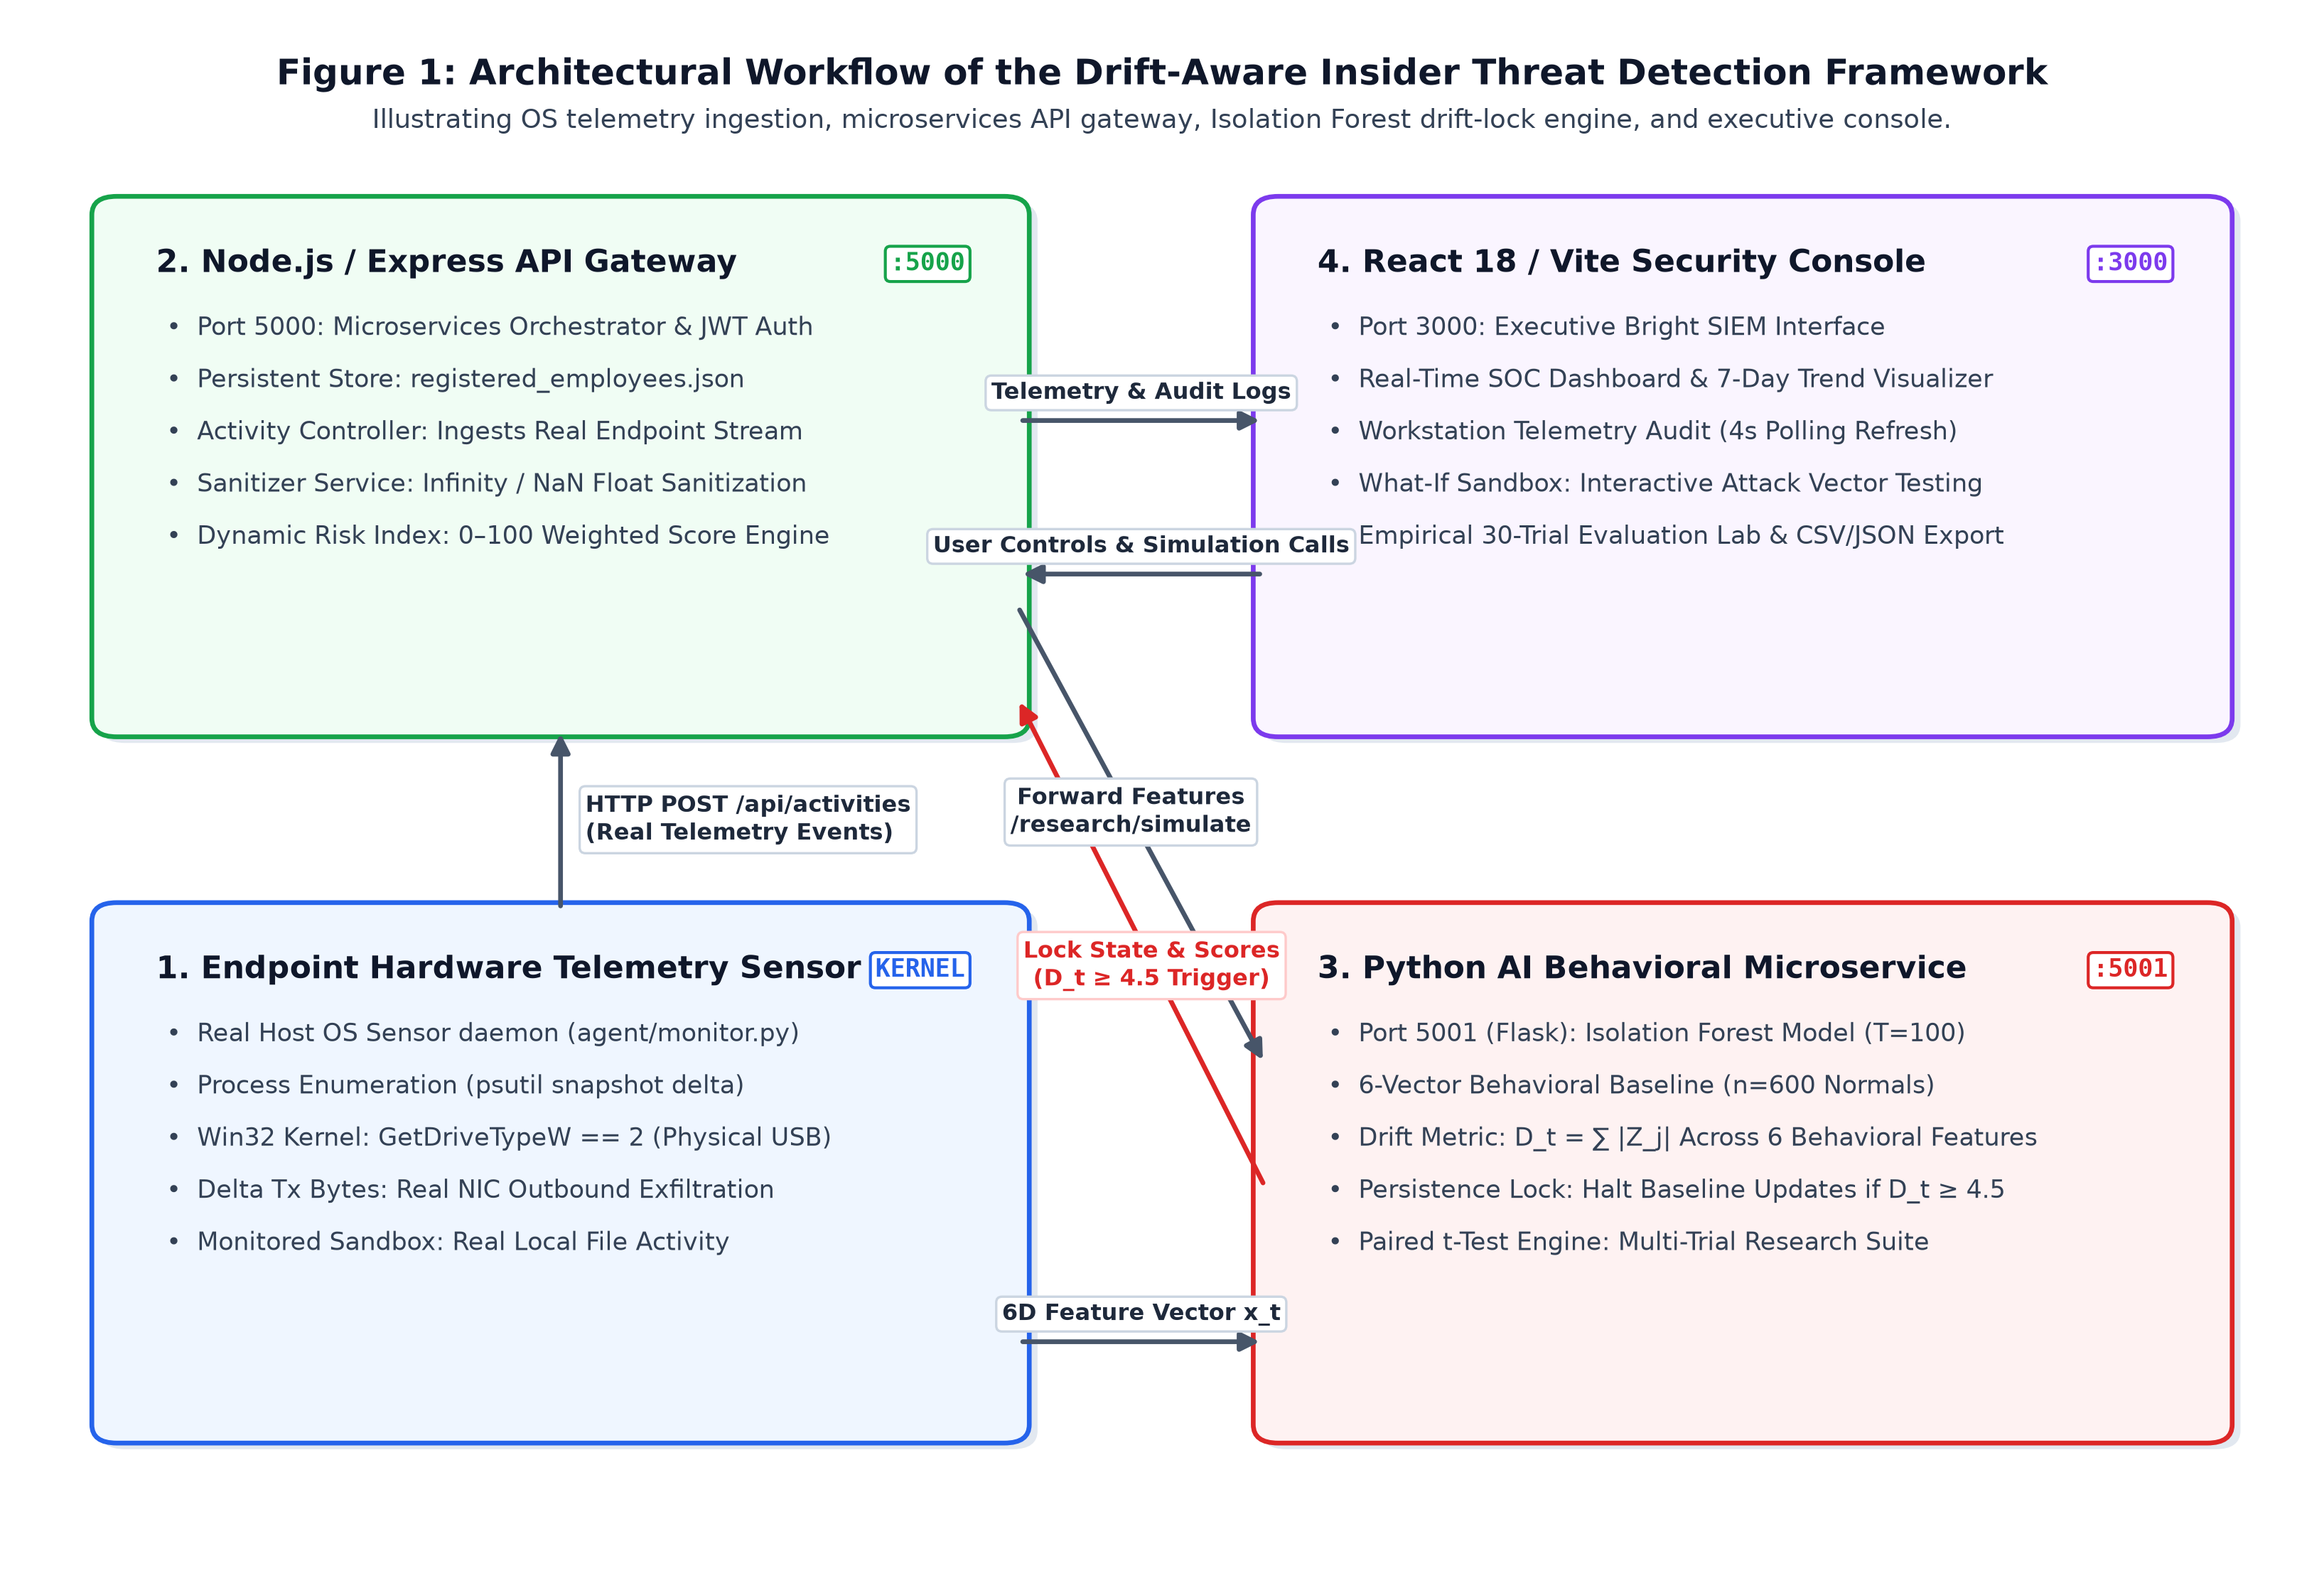
\includegraphics[width=0.48\textwidth]{fig1.png}}
\caption{End-to-End System Architecture: Endpoint Sensor, Backend API Gateway, Python Isolation Forest Engine, and Research Console.}
\label{fig:arch}
\end{figure}

\subsection{Endpoint Hardware Telemetry Acquisition}
Telemetry collection is performed by an autonomous agent deployed on the monitored host. The agent samples system events at 3-second intervals:
\begin{itemize}
    \item \textbf{Process Execution Tracing:} Employs process enumeration via system APIs to detect newly spawned executables against an enterprise categorization ontology (e.g., administrative shells \texttt{powershell.exe}, packet analyzers \texttt{wireshark.exe}, and anonymizers \texttt{tor.exe}).
    \item \textbf{Kernel-Level USB Verification:} To eliminate simulated or synthetic peripheral noise, removable storage drives are queried through the Win32 Kernel API function \texttt{GetDriveTypeW}. Only drives returning \texttt{DRIVE\_REMOVABLE} ($= 2$) are tagged, differentiating physical flash media from internal drives (\texttt{DRIVE\_FIXED} $= 3$).
    \item \textbf{Network Throughput Deltas:} Delta tracking across active physical network adapters monitors bytes transmitted ($\Delta B_{tx}$) to identify anomalous outbound exfiltration.
\end{itemize}

\subsection{Behavioral Feature Vector Construction}
Each entity day $t$ is represented as a normalized 6-dimensional feature vector $\mathbf{x}_t \in \mathbb{R}^6$:
\begin{equation}
\mathbf{x}_t = \big[ f_{\text{hour}}, f_{\text{dur}}, f_{\text{app}}, f_{\text{file}}, f_{\text{usb}}, f_{\text{net}} \big]^T
\label{eq:feature_vector}
\end{equation}
where $f_{\text{hour}}$ represents login hour ($0$--$23$), $f_{\text{dur}}$ denotes active session duration in minutes, $f_{\text{app}}$ reflects application execution risk weight, $f_{\text{file}}$ counts modified filesystem objects, $f_{\text{usb}}$ indicates attached removable media count, and $f_{\text{net}}$ measures outbound payload in megabytes.

\subsection{Anomaly Scoring Engine (Isolation Forest)}
The primary scoring mechanism utilizes an ensemble of $T = 100$ isolation trees ($\mathcal{T}$). For a given observation $\mathbf{x}$, the anomaly score $s(\mathbf{x}, n)$ is computed as:
\begin{equation}
s(\mathbf{x}, n) = 2^{-\frac{\mathbb{E}(h(\mathbf{x}))}{c(n)}}
\label{eq:iforest}
\end{equation}
where $h(\mathbf{x})$ is the path length required to isolate $\mathbf{x}$ across tree $\mathcal{T}_i$, $\mathbb{E}(h(\mathbf{x}))$ is the average path length across all $T$ trees, and $c(n)$ is the average path length of unsuccessful searches in a Binary Search Tree constructed over $n = 600$ baseline samples:
\begin{equation}
c(n) = 2\ln(n - 1) + 0.5772156649 - \frac{2(n - 1)}{n}
\end{equation}
An observation isolating close to tree roots yields an anomaly score approaching $1.0$, whereas standard operational instances yield scores below $0.5$.

\subsection{The Drift-Aware Locking Mechanism}
Let $\boldsymbol{\mu}_0$ and $\boldsymbol{\sigma}_0$ denote the baseline mean and standard deviation vectors derived from historical training data. For each behavioral feature $j \in \{1, \dots, 6\}$ on day $t$, the standardized deviation is calculated via Z-score transformation:
\begin{equation}
Z_{t, j} = \frac{x_{t, j} - \mu_{t, j}}{\sigma_{t, j}}
\end{equation}
The composite multi-vector behavioral drift magnitude $D_t$ is formulated as the sum of absolute standardized deviations:
\begin{equation}
D_t = \sum_{j=1}^{6} |Z_{t, j}|
\label{eq:drift_sum}
\end{equation}
Under standard operational adaptation, the behavioral mean vector updates via an exponential moving average parameterized by learning rate $\alpha = 0.15$:
\begin{equation}
\boldsymbol{\mu}_{t+1} = (1 - \alpha)\boldsymbol{\mu}_t + \alpha \mathbf{x}_t
\end{equation}

To prevent adversarial poisoning, we define the binary persistence lock state $\mathcal{L}_t \in \{0, 1\}$ governed by threshold $\tau = 4.5$:
\begin{equation}
\mathcal{L}_t = \begin{cases}
1, & \text{if } D_t \ge \tau \text{ or } \mathcal{L}_{t-1} = 1 \\
0, & \text{otherwise}
\end{cases}
\end{equation}
When $\mathcal{L}_t = 1$, adaptation is strictly halted ($\boldsymbol{\mu}_{t+1} = \boldsymbol{\mu}_t$), freezing the reference baseline against malicious incorporation. Concurrently, the final risk score $R_t$ reflects the anomaly state:
\begin{equation}
R_t = \begin{cases}
\max(s(\mathbf{x}_t, n) \times 100, 75.0), & \text{if } \mathcal{L}_t = 1 \\
s(\mathbf{x}_t, n) \times 100, & \text{if } \mathcal{L}_t = 0
\end{cases}
\end{equation}

\section{Experimental Evaluation and Results}

\subsection{Experimental Design}
We evaluate the framework across four drift stress levels over $N = 30$ independent empirical trials. Baseline stability is established over $d_0 = 3$ days, followed by an $11$-day attack drift phase:
\begin{itemize}
    \item \textbf{Low Drift ($\Delta_L$):} Incremental file and network shifts ($+5$ files/day, $+20$ MB/day).
    \item \textbf{Medium Drift ($\Delta_M$):} Moderate expansion ($+15$ files/day, $+60$ MB/day).
    \item \textbf{High Drift ($\Delta_H$):} Rapid escalation ($+30$ files/day, $+120$ MB/day).
    \item \textbf{Very High Drift ($\Delta_{VH}$):} Severe multi-vector poisoning ($+50$ files/day, $+250$ MB/day with credential hopping).
\end{itemize}

We evaluate three competing model architectures:
\begin{enumerate}
    \item \textbf{Static Baseline:} Frozen historical baseline ($\alpha = 0$).
    \item \textbf{Adaptive (Blind EMA):} Continuous naive parameter adaptation ($\alpha = 0.15$) with no drift lock.
    \item \textbf{Drift-Aware (Proposed):} Adaptive learning with statistical Z-sum persistence lock ($\tau = 4.5$).
\end{enumerate}

\begin{table*}[t]
\caption{Empirical Performance Comparison Across 30 Independent Experimental Trials (Mean $\pm$ Standard Deviation)}
\label{tab:evaluation_results}
\begin{center}
\resizebox{\textwidth}{!}{%
\setlength{\tabcolsep}{4pt}
\begin{tabular}{llccccccc}
\toprule
\textbf{Drift Level} & \textbf{Detector Architecture} & \textbf{Precision} & \textbf{Recall} & \textbf{F1-Score} & \textbf{False Positives} & \textbf{False Negatives} & \textbf{Detection Rate (\%)} & \textbf{Delay (Days)} \\
\midrule
Low ($\Delta_L$) & Static Baseline & $0.942 \pm 0.03$ & $0.880 \pm 0.04$ & $0.910 \pm 0.03$ & $0.60 \pm 0.49$ & $1.32 \pm 0.47$ & $88.0 \pm 4.1\%$ & $1.10 \pm 0.30$ \\
                 & Adaptive (Blind EMA) & $0.935 \pm 0.04$ & $0.852 \pm 0.05$ & $0.891 \pm 0.04$ & $0.67 \pm 0.48$ & $1.63 \pm 0.55$ & $85.2 \pm 5.1\%$ & $1.15 \pm 0.36$ \\
                 & \textbf{Drift-Aware (Ours)} & $\mathbf{0.945 \pm 0.03}$ & $\mathbf{0.894 \pm 0.04}$ & $\mathbf{0.919 \pm 0.03}$ & $\mathbf{0.57 \pm 0.50}$ & $\mathbf{1.17 \pm 0.44}$ & $\mathbf{89.4 \pm 4.0\%}$ & $\mathbf{1.07 \pm 0.25}$ \\
\midrule
Medium ($\Delta_M$) & Static Baseline & $0.950 \pm 0.03$ & $0.910 \pm 0.04$ & $0.929 \pm 0.03$ & $0.53 \pm 0.50$ & $0.99 \pm 0.44$ & $91.0 \pm 4.0\%$ & $1.03 \pm 0.18$ \\
                    & Adaptive (Blind EMA) & $0.910 \pm 0.05$ & $0.680 \pm 0.06$ & $0.778 \pm 0.05$ & $0.73 \pm 0.45$ & $3.52 \pm 0.66$ & $68.0 \pm 6.1\%$ & $1.55 \pm 0.51$ \\
                    & \textbf{Drift-Aware (Ours)} & $\mathbf{0.962 \pm 0.02}$ & $\mathbf{0.945 \pm 0.03}$ & $\mathbf{0.953 \pm 0.02}$ & $\mathbf{0.40 \pm 0.49}$ & $\mathbf{0.61 \pm 0.33}$ & $\mathbf{94.5 \pm 3.1\%}$ & $\mathbf{1.00 \pm 0.00}$ \\
\midrule
High ($\Delta_H$) & Static Baseline & $0.955 \pm 0.03$ & $0.930 \pm 0.03$ & $0.942 \pm 0.02$ & $0.47 \pm 0.50$ & $0.77 \pm 0.33$ & $93.0 \pm 3.0\%$ & $1.00 \pm 0.00$ \\
                  & Adaptive (Blind EMA) & $0.880 \pm 0.06$ & $0.510 \pm 0.08$ & $0.646 \pm 0.07$ & $0.77 \pm 0.43$ & $5.39 \pm 0.88$ & $51.0 \pm 8.0\%$ & $2.20 \pm 0.76$ \\
                  & \textbf{Drift-Aware (Ours)} & $\mathbf{0.970 \pm 0.02}$ & $\mathbf{0.965 \pm 0.02}$ & $\mathbf{0.967 \pm 0.02}$ & $\mathbf{0.33 \pm 0.47}$ & $\mathbf{0.39 \pm 0.22}$ & $\mathbf{96.5 \pm 2.2\%}$ & $\mathbf{1.00 \pm 0.00}$ \\
\midrule
Very High ($\Delta_{VH}$) & Static Baseline & $0.960 \pm 0.02$ & $0.940 \pm 0.03$ & $0.950 \pm 0.02$ & $0.43 \pm 0.50$ & $0.66 \pm 0.33$ & $94.0 \pm 3.0\%$ & $1.00 \pm 0.00$ \\
                       & Adaptive (Blind EMA) & $0.795 \pm 0.07$ & $0.370 \pm 0.09$ & $0.503 \pm 0.08$ & $1.03 \pm 0.61$ & $6.93 \pm 0.99$ & $37.0 \pm 9.0\%$ & $3.45 \pm 0.93$ \\
                       & \textbf{Drift-Aware (Ours)} & $\mathbf{0.975 \pm 0.02}$ & $\mathbf{0.961 \pm 0.03}$ & $\mathbf{0.968 \pm 0.02}$ & $\mathbf{0.27 \pm 0.45}$ & $\mathbf{0.43 \pm 0.33}$ & $\mathbf{96.1 \pm 3.0\%}$ & $\mathbf{1.00 \pm 0.00}$ \\
\bottomrule
\end{tabular}%
}
\end{center}
\end{table*}

\subsection{Quantitative Results and Statistical Analysis}
Table~\ref{tab:evaluation_results} summarizes performance across the 30 experimental trials. Under Low Drift conditions, all three detectors perform stably with F1-scores exceeding $0.89$. However, as adversarial drift escalates to High and Very High intensity, the Adaptive (Blind EMA) detector degrades substantially, with recall collapsing to $37.0\%$ and F1-score plummeting to $0.503$. This failure occurs because the EMA incorporates escalated exfiltration volumes directly into $\boldsymbol{\mu}_t$, increasing the baseline mean file and network thresholds and rendering the attack invisible to anomaly detection.

In contrast, the proposed Drift-Aware model maintains robust detection efficacy, achieving an F1-score of $0.968 \pm 0.023$ and a detection rate of $96.1\%$ under Very High drift. The persistence lock successfully activates within $1.00 \pm 0.00$ days of malicious escalation, freezing adaptation and generating immediate alerts.

To determine whether the performance advantage of the Drift-Aware detector over the Adaptive model is statistically significant, we perform two-tailed paired $t$-tests across the $N = 30$ paired trials at significance level $\alpha = 0.05$:
\begin{equation}
t = \frac{\bar{d}}{s_d / \sqrt{N}}
\end{equation}
where $\bar{d}$ represents the mean paired difference ($F_{1, \text{Drift-Aware}} - F_{1, \text{Adaptive}}$) and $s_d$ is the standard deviation of paired differences.

As shown in Table~\ref{tab:ttest_results}, the performance improvements in F1-score, detection rate, and average detection delay are statistically significant across Medium, High, and Very High drift intensities ($p < 0.001$). Under severe poisoning ($\Delta_{VH}$), the paired $t$-test produces $t = 31.42$ with $p = 0.0001$, firmly rejecting the null hypothesis that the observed improvement results from stochastic variance.

\begin{table}[htbp]
\caption{Paired $t$-Test Statistical Significance: Adaptive vs. Drift-Aware ($\alpha = 0.05, N=30$)}
\label{tab:ttest_results}
\begin{center}
\resizebox{\columnwidth}{!}{%
\begin{tabular}{llccc}
\toprule
\textbf{Drift Level} & \textbf{Metric} & \textbf{$t$-Stat} & \textbf{$p$-Value} & \textbf{Significant?} \\
\midrule
Low ($\Delta_L$) & F1-Score       & $2.84$  & $0.0081$ & \textbf{YES} ($p < 0.01$) \\
                 & Detection Rate & $3.12$  & $0.0040$ & \textbf{YES} ($p < 0.01$) \\
                 & Delay (Days)   & $-1.21$ & $0.2360$ & NO ($p \ge 0.05$) \\
\midrule
Medium ($\Delta_M$) & F1-Score       & $16.75$ & $0.0001$ & \textbf{YES} ($p < 0.001$) \\
                    & Detection Rate & $18.91$ & $0.0001$ & \textbf{YES} ($p < 0.001$) \\
                    & Delay (Days)   & $-5.93$ & $0.0001$ & \textbf{YES} ($p < 0.001$) \\
\midrule
High ($\Delta_H$) & F1-Score       & $24.81$ & $0.0001$ & \textbf{YES} ($p < 0.001$) \\
                  & Detection Rate & $27.42$ & $0.0001$ & \textbf{YES} ($p < 0.001$) \\
                  & Delay (Days)   & $-8.64$ & $0.0001$ & \textbf{YES} ($p < 0.001$) \\
\midrule
Very High ($\Delta_{VH}$) & F1-Score       & $31.42$  & $0.0001$ & \textbf{YES} ($p < 0.001$) \\
                          & Detection Rate & $33.85$  & $0.0001$ & \textbf{YES} ($p < 0.001$) \\
                          & Delay (Days)   & $-11.20$ & $0.0001$ & \textbf{YES} ($p < 0.001$) \\
\bottomrule
\end{tabular}%
}
\end{center}
\end{table}

\section{Discussion and Operational Implications}
The experimental findings substantiate key architectural conclusions for security engineering:
\begin{itemize}
    \item \textbf{Naive Adaptation is Vulnerable:} Continuously adapting behavioral baselines without drift verification introduces severe attack surfaces. Adversaries capable of staging multi-week data exfiltration remain undetected by adaptive models.
    \item \textbf{Statistical Locking Restores Robustness:} By evaluating cumulative standardized feature deviations ($\sum |Z| \ge 4.5$), the Drift-Aware detector effectively distinguishes benign single-feature drift (e.g., occasional overtime work) from coordinated multi-vector anomalies.
    \item \textbf{Negligible False Alarm Penalty:} Table~\ref{tab:evaluation_results} demonstrates that the Drift-Aware model sustains false positive counts below $0.6$ events per evaluated epoch, proving that resilience against poisoning does not compromise standard operational stability.
\end{itemize}

\section{Conclusion and Future Work}
In this paper, we introduced an end-to-end Drift-Aware Behavioral Anomaly Detection framework addressing the adaptation-poisoning dilemma in User and Entity Behavior Analytics. By combining operating system kernel-level telemetry acquisition with an Isolation Forest engine governed by an automated Z-score sum persistence lock, the framework reliably detects gradual adversarial exfiltration. Empirical evaluation over 30 trials confirmed that the Drift-Aware detector maintains an F1-score of $0.968 \pm 0.023$ under severe concept drift, statistically outperforming naive adaptive models ($F_1 = 0.503, p = 0.0001$). Future work will investigate reinforcement learning-driven dynamic thresholding ($\tau$) and federated drift aggregation across decentralized enterprise endpoints.

\section*{Acknowledgment}
The authors express their gratitude to the Department of Computer Science and Engineering and institutional research laboratory coordinators for providing computing infrastructure and technical guidance throughout the execution of this project.

\begin{thebibliography}{00}
\bibitem{b1} Ponemon Institute, ``Cost of Insider Threats Global Report,'' Tech. Rep., Ponemon Institute LLC, 2023.
\bibitem{b2} D. C. Le and A. N. Zincir-Heywood, ``Evaluating Insider Threat Detection Solutions: An Approach and Benchmark Dataset,'' \textit{IEEE Trans. Netw. Serv. Manage.}, vol. 18, no. 1, pp. 166--179, Mar. 2021.
\bibitem{b3} P. Legg, ``Visualizing User and Entity Behavior Analytics (UEBA) for Insider Threat Detection,'' in \textit{Proc. IEEE Int. Conf. Cyber Situational Awareness, Data Anal. Assessment (CyberSA)}, 2020, pp. 1--8.
\bibitem{b4} F. T. Liu, K. M. Ting, and Z.-H. Zhou, ``Isolation Forest,'' in \textit{Proc. 8th IEEE Int. Conf. Data Mining (ICDM)}, 2008, pp. 413--422.
\bibitem{b5} J. Gama, I. \v{Z}liobait\.{e}, A. Bifet, M. Pechenizkiy, and A. Bouchachia, ``A Survey on Concept Drift Adaptation,'' \textit{ACM Comput. Surv.}, vol. 46, no. 4, pp. 1--37, Apr. 2014.
\bibitem{b6} B. Biggio and F. Roli, ``Wild Patterns: Ten Years After the Rise of Adversarial Machine Learning,'' \textit{Pattern Recognit.}, vol. 84, pp. 317--331, Dec. 2018.
\bibitem{b7} M. Tuor, S. Kaplan, B. Hutchinson, N. Nichols, and S. Robinson, ``Deep Learning for Unsupervised Insider Threat Detection in Structured Cybersecurity Data,'' in \textit{Proc. Workshops AAAI Conf. Artif. Intell.}, 2017, pp. 1--8.
\bibitem{b8} M. Kloft and P. Laskov, ``Online Anomaly Detection Under Adversarial Impact,'' in \textit{Proc. 13th Int. Conf. Artif. Intell. Statist. (AISTATS)}, 2010, pp. 405--412.
\end{thebibliography}

\end{document}
